
\section{Introduction}
\label{sec:introduction}
\begin{figure*}[ht]
	\centering
	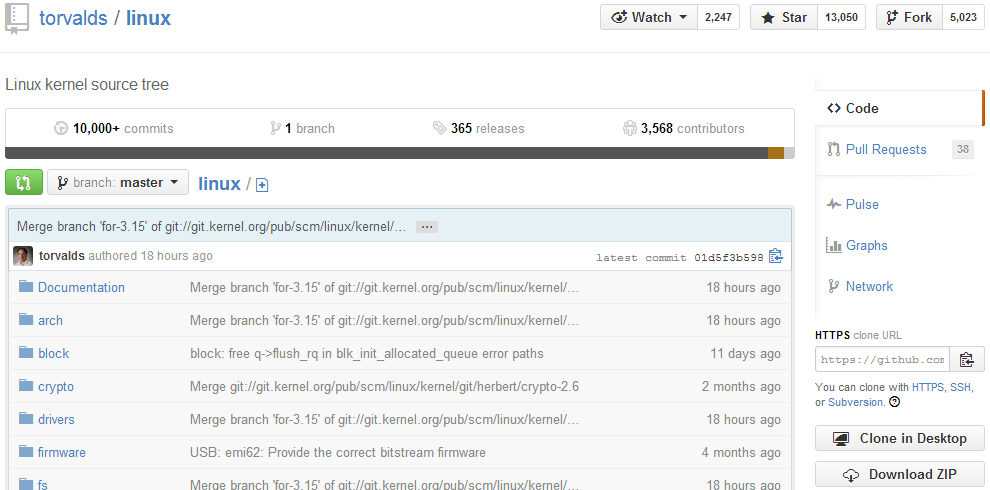
\includegraphics[width=0.98\textwidth]{./img/linux.png}
	\caption{Sample profile of a repository in GitHub}
	\label{fig:ghrepo}
\end{figure*}
With the advent of Web 2.0, online collaboration has become not only a part of internet experience but rather a necessity. People today are not just passive viewers of content but rather active contributors. Social networking sites such as Facebook and LinkedIn allow users to create both their personal and professional identities, respectively. Further, online communities such as blogs and wikis allow people to express opinions, carry out discussions, ask questions and answer queries, among other things. In addition, media sharing and hosting websites such as YouTube ensure fast propagation and easy accessibility of digital content.

Clearly, digital collaborations have revolutionized the way information is generated (i.e. through multiple sources), stored (social graphs and complex data types) and accessed (fast and ubiquitous) using just a web browser. This is also true for software development. Recently, platforms such as SourceForge, GitHub, BitBucket and CodePlex have experienced a rise in popularity. They are also referred to as social coding platforms i.e. development environment that encourages formal and informal collaboration on software projects providing opportunities for discussion and sharing. Open Source Software (OSS) in particular has experienced a rise in popularity. These open source projects are licensed to be freely modified and distributed and hence are often developed publicly where multiple developers collaborate to add or modify functionality.

The social aspects of OSS development provides insight into the dynamics of collaborations and opens interesting opportunities for research. Several studies throw light on what drives people towards OSS. Some of these factors include personal need for software \cite{Raymond1999}, creative stimulation \cite{lakhani2005}, learning \cite{Lakhani2003}, gift-giving intentions \cite{Zeitlyn2003} and significant returns on contribution \cite{ghosh2005}. Even though the developers have these intentions in mind, they seldom have any explicit metric to measure such factors. In the absence of such information developers indirectly assess the reputation of a project or a developer based on several other factors. For instance, number of followers of a developer can be indicative of their reputation in the coding community.

In this paper we will focus on collaborations between software developers, ``Social Coding'' and OSS development. We will discuss how these collaborations function by analysing one of the most popular social coding website - GitHub \cite{GitHub}. We are particularly interested in studying what motivates a developer to contribute into a project. The large amount of projects that a developer can join and contribute seems overwhelming. Yet, somehow, some of the projects seem to be more attractive to developers and have larger communities that are willing to  contribute to their development. A simple intuition of this phenomenon would be that popular projects attract developers simply because they are popular, like a snowball effect.

While this might be true for some projects, various counterexamples can be found in which a project quickly gathers a significant following, with no obvious reason. Our study will focus on analyzing the social network of GitHub and provide some answers to the following questions:

\textbf{Q1:} What is a typical contributor of a project?

\textbf{Q2:} Why do people follow specific projects?

We believe that by answering these questions we can help developers build a following to their projects. The remainder of our paper is structured as follows: In section 2 we will discuss similar factors that can affect collaboration decisions and reputation by reviewing some of the previous work that has been done in the field. Section 3 presents the data collected from Github and use it to answer Q1. In section 4, we analyze some trends on the data and use them to answer Q2. In section 5, we discuss some threats to the validity of our work. Finally, in section 6 we present our conclusions.
